\section{Auswertung und Diskussion der Messwerte}
\label{sec:Auswertung}

\subsubsection{Dämpfungswiderstand}
\begin{figure}
  \centering
  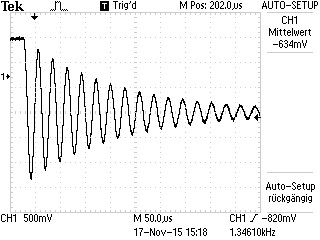
\includegraphics{data/F0000TEK.jpg}
  \caption{zeitlicher Spannungsverlauf}
  \label{fig:5aergebnis}
\end{figure}
Abb. \ref{fig:5aergebnis} zeigt den Verlauf der Spannung in dem gedämpften
Schwingkreis. Qualitaiv gut zu erkennen sind die sinusförmige Schwingung und
die einhüllende e-Funktion, die die Dämpfung beschreibt.
Die Frequenz beträgt 1,35 kHz.
Die Maxima der Spannungen sind in folgender Tabelle dargestellt:
\begin{table}
\noindent
\caption{Messwerte 5a)}
\label{tab:5a}
\sisetup{table-format=1.2}
\begin{tabular}{ll}
\toprule
{$t$[s]} & {$U$[V]} \\
\midrule
-0.0000206 & 0.78 \\
-0.0000058 & -2.06 \\
0.0000078 & 0.54 \\
0.00002260 & -1.88 \\
0.00003700 & 0.36 \\
0.00005160 & -1.70 \\
0.00006600 & 0.18 \\
0.00008100 & -1.56 \\
0.00009500 & 0.08 \\
0.00010980 & -1.44 \\
0.00012500 & -0.04 \\
0.00013800 & -1.34 \\
0.00015240 & -0.14 \\
0.00016760 & -1.24 \\
0.00018160 & -0.22 \\
0.00019660 & -1.18 \\
0.00021020 & -0.30 \\
0.00022640 & -1.12 \\
0.00023860 & -0.36 \\
0.00025420 & -1.06 \\
0.00026800 & -0.42 \\
0.00028240 & -1.02 \\
\bottomrule
\end{tabular}
\end{table}

Der negative Zeitabschnitt bei den ersten beiden Messwerten
sowie die Tatsache, dass
die Messwerte der Spannung
in positiver und negativer Hinsicht nicht übereinstimmen,
spielen für die Berechnung des Dämpfungswiderstandes keine größere Rolle
(siehe Diskussion).
Als Spannungsamplitude wird im folgenden die Differenz zwischen Maximum und
Minimum der Spannung bezeichnet, auf \ref{tab:5a} bezogen also jeweils die
Differenz zweier aufeinanderfolgenden Werte.
Der Abfall der Spannung soll der Theorie
zufolge(siehe Gleichung \ref{eqn:Ischwingung})
mit $e^{-2\pi\mu t}$ erfolgen. Die Spannungsamplitude fällt unter
$\frac{1}{e}$tel des ursprünglichen Wertes bei t=0.0001816 s.
Da der erste Messwert
nicht bei t=0 aufgenommen wurde, ergibt sich also $T_{ex}$ = 0.2022ms.
Der Exponent der e-Funktion muss zu diesem Zeitpunkt -1 betragen (auf 4$/e=e^-1$
abgefallen), es ergibt sich also:
\begin{equation}
  -2\pi\mu T_{ex} = -1 \\
  \implies \mu = \frac{1}{2\pi T_{ex}} = 787,11 \text{1/s.}
\end{equation}

\subsubsection{Aperiodischer Grenzfall)}
\begin{figure}
  \centering
  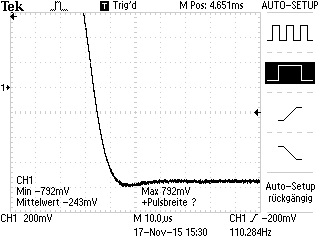
\includegraphics{data/F0001TEK.jpg}
  \caption{aperiodischer Grenzfall}
  \label{fig:5bergebnis}
\end{figure}

Abb. \ref{fig:5bergebnis} zeigt den gemessenen Spannungsabfall für
R = 3120 $\Omega$.
Bei diesem Widerstand tritt die aperiodische Dämpfung auf, was daran zu erkennen
ist dass kein Überschwingen stattfindet wie z.B. in Abb.\ref{fig:über}
(R=2260$\Omega$).
\begin{figure}
  \centering
  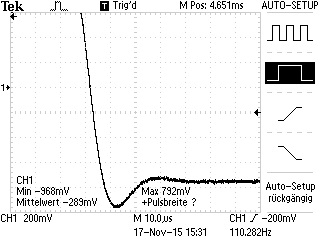
\includegraphics{data/F0002TEK.jpg}
  \caption{aperiodische Dämpfung mit $R \neq R_{ap}$}
  \label{fig:über}
\end{figure}

Der theoretische Wert berechnet sich gemäß:
\begin{equation}
  \frac{1}{LC} = R_{ap}^2/4L^2 \\
  \implies R_{ap} = \sqrt{\frac{4L}{C}} = 4390.4 \pm 9.0\Omega.
\end{equation}

Der theoretische Wert weicht recht deutlich (\~40\%) von dem gemessenen ab.
Eine Erklärung dafür könnten die weiteren internen Widerstände sein, die in
der Schaltung in Form von Kabel u.ä. enthalten sind. Außerdem ist der Fehler
des regelbaren Widerstandes nicht bekannt. Zusätzlich zu der Ableseungenauigekeit
können durchaus noch einige Prozentpunkte durch diesen Faktor dazukommen.
Ohne Genaueres über den verwendeten Widerstand zu wissen, erscheint die
Abweichung vom Theoriewert allerding recht hoch und lässt einen Fehler
bei der Messung vermuten.

\subsubsection{Resonanzüberhöhung)}
\label{sec:5c}
Um die Resonanzüberhöhung zu bestimmen, wird zunächst die Kondensatorspannung
relativ zu der Erregerspannung berechnet. Da beide Werte mit dem selben Tastkopf
gemessen wurden, kann die Frequenzabhängigkeit dieses vernachlässigt werden
und man erhält $U_{rel}=\frac{U_c}{U_0}$. Die Messwerte sind in folgender
Tabelle dargestellt:
\begin{table}
\centering
\caption{Messwerte 5c)}
\label{tab:5b}
\sisetup{table-format=1.2}
\begin{tabular}{lll}
\toprule
{$U_c$[V]} & {$U_0$[V]} &{$f$[kHz]}\\
\midrule
1.28 & 1.44 & 4.26 \\
1.48 & 1.45 & 6.00 \\
1.51 & 1.44 & 8.00 \\
1.56 & 1.44 & 10.00 \\
1.60 & 1.45 & 12.00 \\
1.71 & 1.44 & 14.00 \\
1.80 & 1.48 & 16.00 \\
1.93 & 1.48 & 18.00 \\
2.10 & 1.48 & 20.00 \\
2.33 & 1.48 & 22.00 \\
2.60 & 1.48 & 24.00 \\
3.00 & 1.48 & 26.00 \\
3.50 & 1.48 & 28.00 \\
4.28 & 1.52 & 30.00 \\
4.96 & 1.48 & 32.00 \\
5.52 & 1.38 & 34.00 \\
4.92 & 1.38 & 36.00 \\
4.08 & 1.44 & 38.00 \\
3.20 & 1.48 & 40.00 \\
\bottomrule
\end{tabular}
\end{table}
\begin{figure}
  \centering
  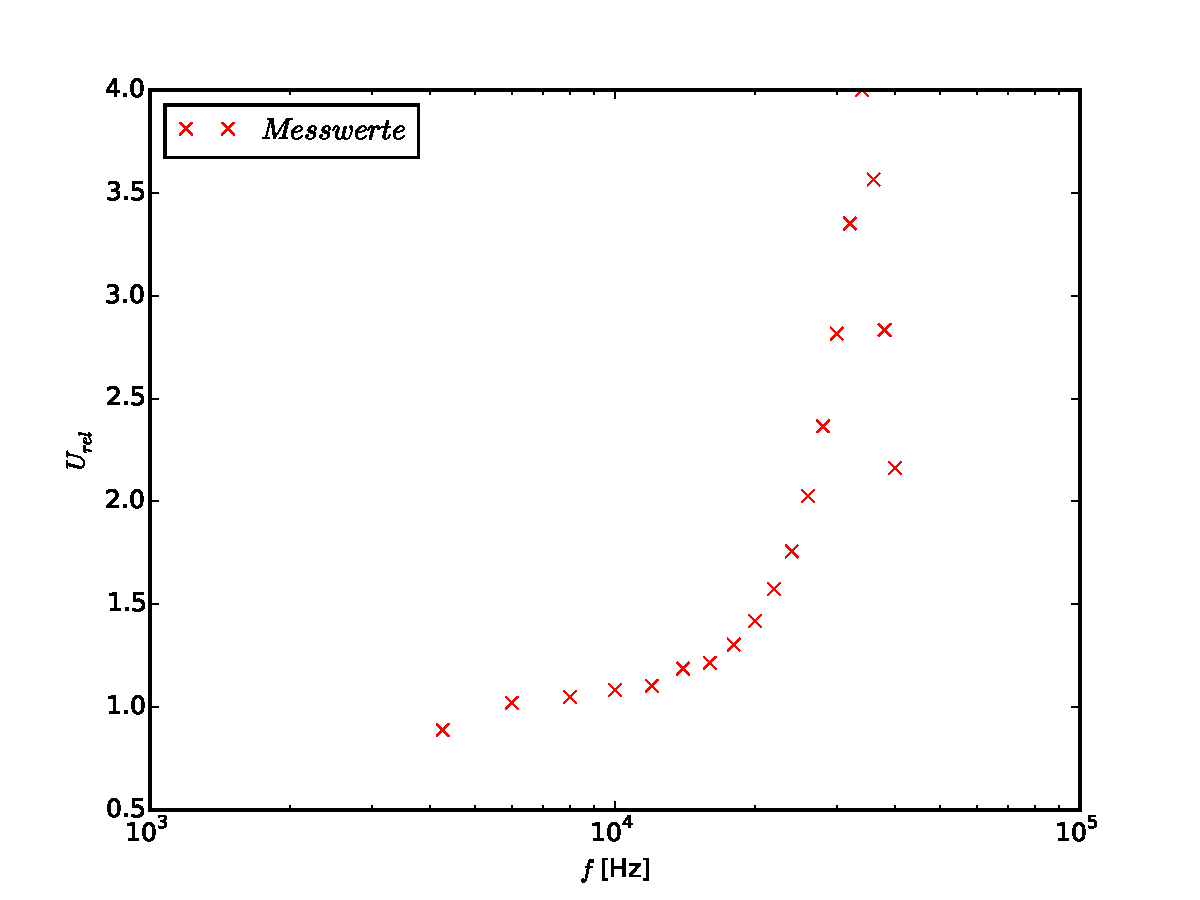
\includegraphics[width=\textwidth]{5c.pdf}
  \caption{Halblogarithmischer Plot}7
  \label{fig:5cergebnis}
\end{figure}
In Abb.\ref{fig:5cergebnis} lässt sich das qualitativ erwartete Ergebnis
wiederfinden: Um die Resonanzfrequenz $\omega_0$ steigt die Kondensatorspannung
sprunghaft an, für geringe Frequenzen nähert sie sich der Erregerspannung $U_0$.
Auffällig ist der Wert bei $f=4,26$kHz, bei dem die Kondensatorspannung unter
$U_0$ fällt. Dies ist mit der Theorie nicht vereinbar und am ehesten auf einen
Fehler bei der Messung von $U_c$ zurückzuführen. Die maximale Spannung liegt
bei $4\cdot U_0$, womit die Resonanzüberhöhung bei exakt 4 liegt.

Zur Bestimmung der Schärfe der Resonanz ist es zweckmäßig den Bereich um die
Resonanzfrequenz linear darzustellen, so zu sehen in Abb.\ref{fig:5clin}
\begin{figure}
  \centering
  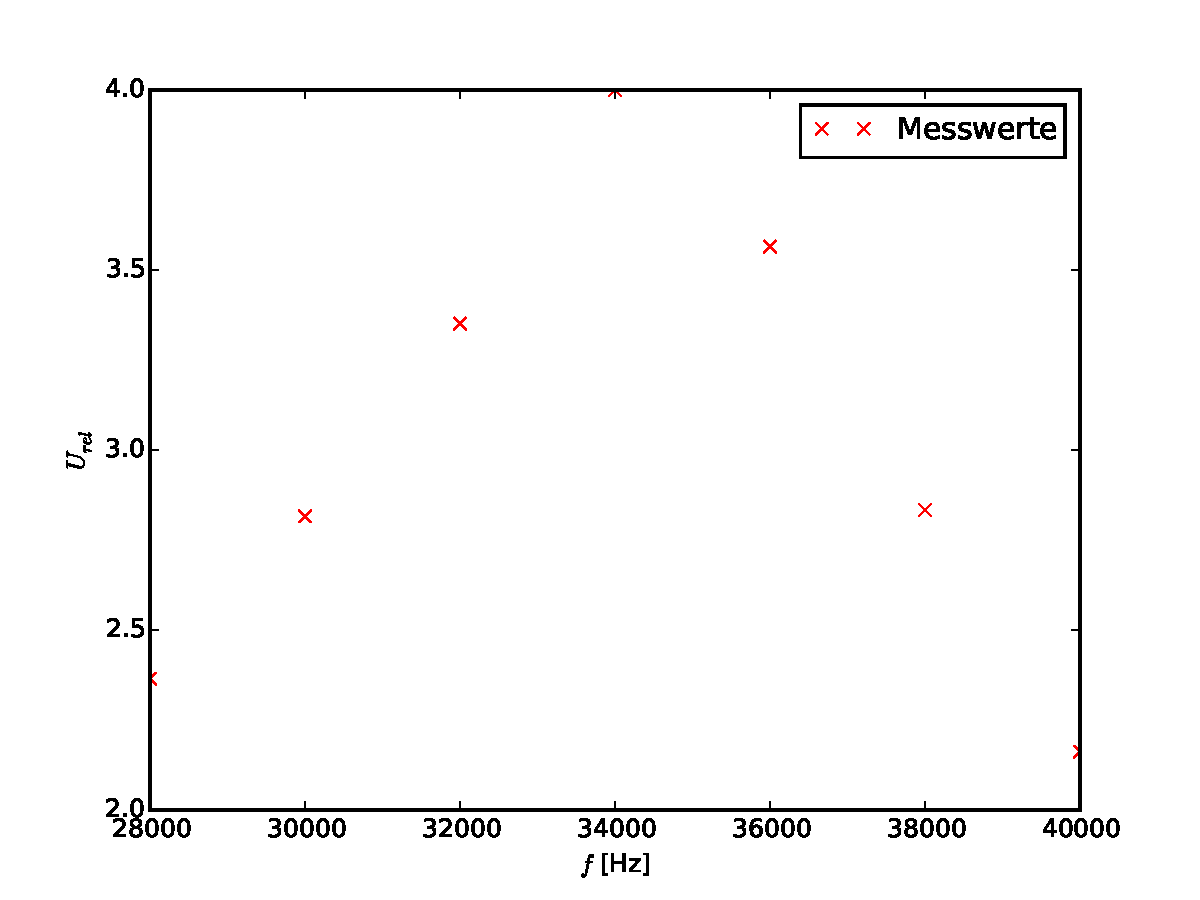
\includegraphics[width=\textwidth]{5c2.pdf}
  \caption{$U_{rel}$ im Bereich der Resonanzfrequenz}
  \label{fig:5clin}
\end{figure}
Die Resonanzfrequenz liegt im Rahmen der aufgenommenen Messwerte bei
$\omega$ = 34 kHz.
In vorliegendem Fall entspricht $U_{rel}(\omega_{\pm})$ dem 2.83 fachen von $U_0$.
Diese Werte werden ziemlich genau bei $\omega_-$ = 30 kHz ($U_{rel}=2.82$) und
$\omega_+$=38kHz ($U_{rel} = 2.83$) erreicht. Gemäß Gleichung \ref{eqn:güte2} ergibt
sich demnach für die Güte:
$q = \frac{34}{38-30} = \frac{34}{8} = 4.25$ (Einheiten für $\omega$ gekürzt).
Dieser Wert weicht nur um 6,25\% von dem Wert ab, der aus der maximalen
Spannung hergeleitet wurde. Die Abweichung lässt sich neben Messfehlern in erster
Linie auf die geringe Anzahl an Messwerten im Bereich der Resonanzfrequenz
zurückführen. Dadurch ist die Genauigkeit bei der Bestimmung von
$U_{Cmax}$ sowie $\omega_\pm$ begrenzt. Die maximale Spannung kann durchaus
einige Prozentpunkte höher als der höchste gemessene Wert von $4\cdot U_0$
liegen.
Berechnet man die Güte anhand der Parameter des Schwingkreises
(Vgl. \ref{eqn:güte1}) erhält man mit: \\
$L = 10,11 \pm 0,03$ mH \\
$C = 2,098 \pm 0,006$ nF und \\
$R = 509,5 \pm 0,5 \Omega$\\
für die Güte:
$q = 4.309 \pm 0.010$.
Dieser Wert liegt in guter Übereinstiimmung mit den beiden aus den Messwerten
erhaltenen Werten für q.

\subsubsection{Phasenverschiebung}
Die Messwerte für $\phi$ sind in folgender Tabelle auffgelistet, Abb.
\ref{fig:5dlog} zeigt $\phi$ in Abhängigkeit von der Frequenz $f$ mit
logarithmischer x-Achse, Abb.\ref{fig:5dlin} den Bereich um $\phi$ = 90° mit
linearen Achsenskalierungen.
\begin{table}
\centering
\caption{Messwerte 5c)}
\label{tab:5c}
\sisetup{table-format=1.2}
\begin{tabular}{rr}
\toprule
{$\phi$[deg]} &{$f$[kHz]}\\
\midrule
7.67 & 4.26 \\
6.48 & 6.00 \\
3.46 & 8.00 \\
1.44 & 10.00 \\
5.18 & 12.00 \\
6.05 & 14.00 \\
10.37 & 16.00 \\
12.96 & 18.00 \\
11.52 & 20.00 \\
19.01 & 22.00 \\
17.28 & 24.00 \\
22.46 & 26.00 \\
32.26 & 28.00 \\
45.36 & 30.00 \\
57.6 & 32.00 \\
80.78 & 34.00 \\
108.86 & 36.00 \\
125.86 & 38.00 \\
141.12 & 40.00 \\
\bottomrule
\end{tabular}
\end{table}

\begin{figure}
  \centering
  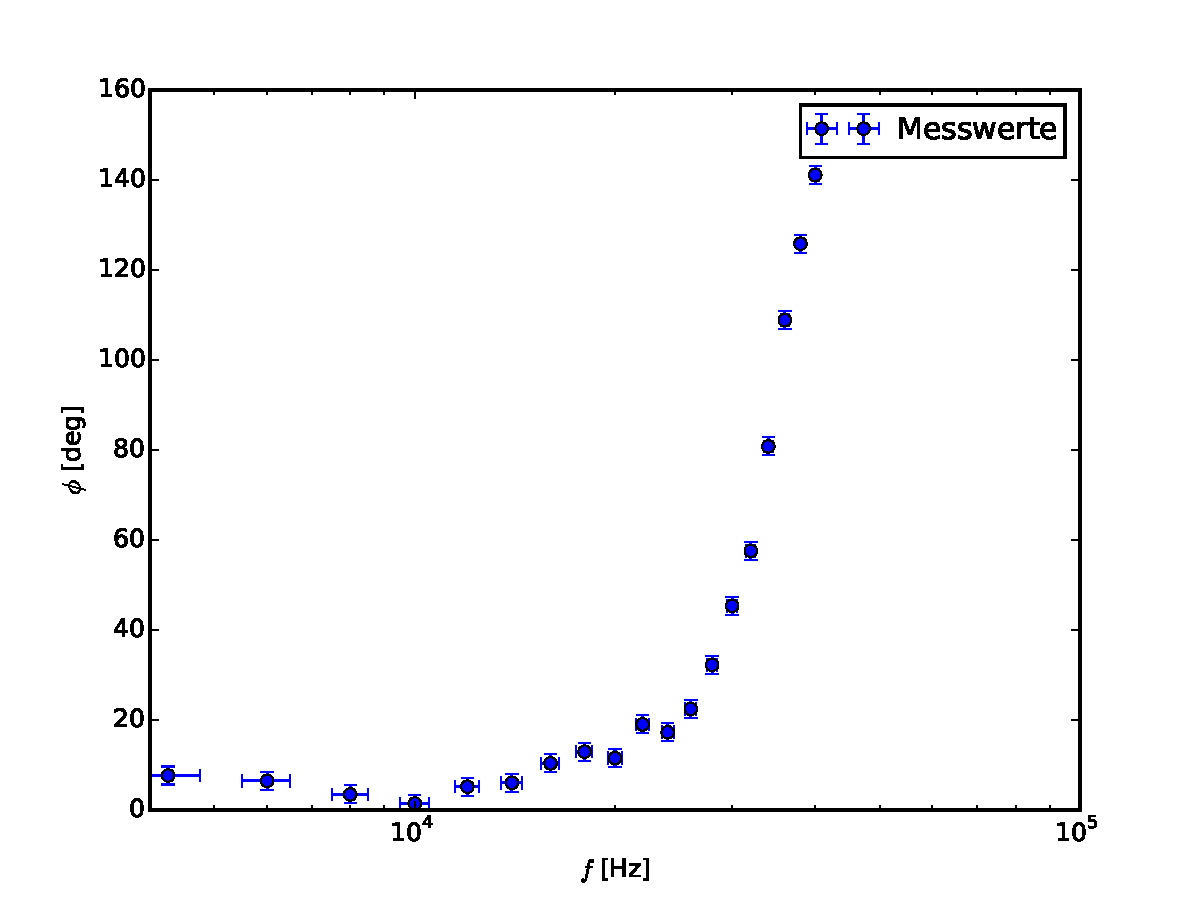
\includegraphics[width=\textwidth]{5d.pdf}
  \caption{$\phi$ mit halblogarithmischer Achseneinteilung}
  \label{fig:5dlog}
\end{figure}

\begin{figure}
  \centering
  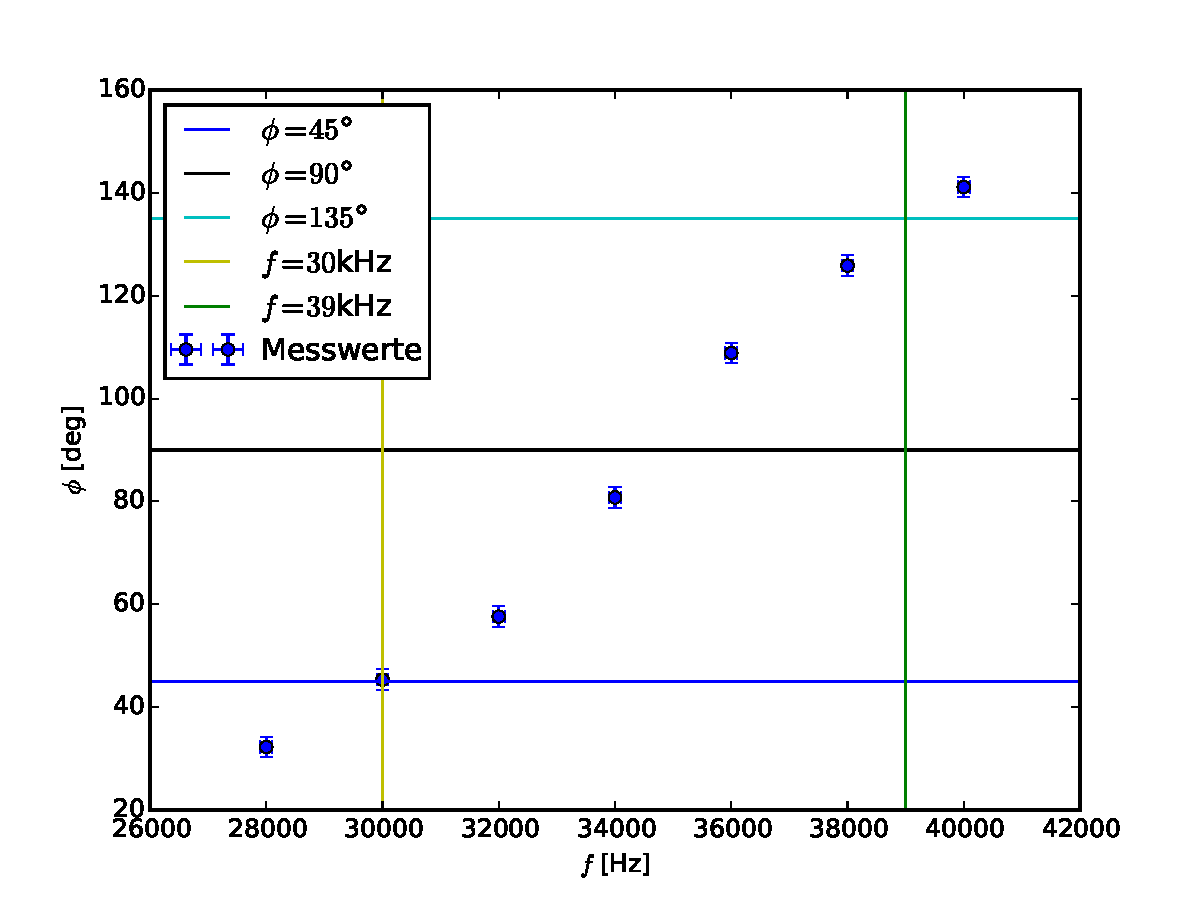
\includegraphics[width=\textwidth]{5d2.pdf}
  \caption{$\phi$ im Bereich der Resonanzfrequenz}
  \label{fig:5dlin}
\end{figure}

In Abb. \ref{fig:5dlin} sind außerdem die Geraden eingetragen um das Ablesen
der relevanten Phasenverschiebungen zu erleichtern.
$\omega_1$ ($\phi$ = 45°) liegt ziemlich fast exakt bei 30kHz ($\phi$=45,36°),
$\omega_2$ liegt bei \~ 39kHz. Damit liegen $\omega_1$ und $\omega_2$ bei
ähnlichen Frequenzen wie zuvor (Vgl. Abschnitt \ref{sec:5c}) schon $\omega_-$
und $\omega_+$ Dies ist das erwartete Ergebnis für den Fall schwacher
Dämpfung, der hier realisiert ist. $\omega_1$ und $\omega_-$ sind im Rahmen
der begrenzten Anzahl an Messwerten identisch, $\omega_2$ und $\omega_+$ weichen
um \~13\% voneinander ab.
